\documentclass[journal,comsoc]{IEEEtran}

\usepackage[T1]{fontenc}% optional T1 font encoding
\usepackage{cite}
\usepackage[pdftex]{graphicx}
\usepackage{epstopdf}
\usepackage{amsmath}
\usepackage[caption=false,font=footnotesize]{subfig}
\newcommand{\hbAverage}[1]{\overline{#1}}
\newcommand{\etal}{et al. }
\newcommand{\hbie}{i.e.,}
\newcommand{\hbeg}{e.g.,}
\newcommand{\hbSection}[1]{\section{#1}}
\newcommand{\hbQuote}[1]{``\textsf{{\footnotesize #1}}''}
\usepackage{color}
\newcommand{\hbIdea}[1]{{\color{red}{\scriptsize [{#1}]}}}
\newcommand{\myFigWidth}{8cm}
\usepackage[hidelinks]{hyperref}
\newcommand{\reffig}[1]{Fig.~\ref{#1}}
\newcommand{\refeq}[1]{Eq.~\ref{#1}}
\newcommand{\reftbl}[1]{Table~\ref{#1}}
\newcommand{\refsec}[1]{Sec.~\ref{#1}}
\newcommand{\refthm}[1]{Theorem~\ref{#1}}
\newcommand{\refthmA}[2]{\refthm{#1}(\ref{#2}}
\newcommand{\reflem}[1]{Lemma~\ref{#1}}
\newcommand{\refdef}[1]{Definition~\ref{#1}}
\newcommand{\refexmp}[1]{Example~\ref{#1}}
\newcommand{\refitem}[1]{(\ref{#1})}
\newcommand{\refcite}[1]{ref~\cite{#1}}
\usepackage[iso]{datetime}
\newcommand{\hbNow}{--Draft-- v\today/\currenttime} % version


\hyphenation{op-tical net-works semi-conduc-tor}


\begin{document}


\title{
	Smart presentation of HTML pages
}

\author{Kerim Can Macit}
% \thanks{
% H.~O.~Bingol  and Omer Basar are with 
% the Department of Computer Engineering, 
% Bogazici University, 
% Istanbul,
% 34342 Turkey 
% e-mail: bingol@boun.edu.tr.
% }% <-this % stops a space
% \thanks{Manuscript received December 1, 2015; revised XX XX, 2015.}}


\maketitle


% \begin{abstract}
% 	ABSTRACT WILL BE HERE
% \end{abstract}


% \begin{IEEEkeywords}
% 	HTML,
% 	Presentation,
% 	Markdown
% \end{IEEEkeywords}


\IEEEpeerreviewmaketitle


\section{Introduction}

\IEEEPARstart{T}{here} 
%Using 
are several options and plenty of dedicated software for generating presentations, from Microsoft PowerPoint to web services, like Prezi. Each option has some advantages and disadvantages over others. In this project, I will research on HTML page usage for presentation and implement navigation handler for presentation purposes.

HTML pages for presentation has some advantages over traditional presentation software. The most dominant advantage of HTML presentation is that it does not require any special software in order to present. Any device with basic internet browser will be able to handle HTML presentation which makes it platform independent. 

HTML pages also give more flexibility compared to traditional ones. Also, most popular presentation programs requires subscription in order to use. Also, with some programming knowledge, structure and navigation tool can easily be change.

HTML pages are also tends to be smaller in size. Therefore, it has some advantage in publishing and sharing the presentation.

Although having some advantages, generating HTML pages for presentation requires some technical knowledge. Therefore, in this application, I will use some type of markdown to HTML converter in order to make it easy for the presenter or presentation generator.

% =========================================================================
\section{System Description}

Basically, the system can be explained as HTML page presentation app. App has 3 main features, mark-down to HTML generator, presentation ordering part and lastly navigation system.

The aim of MD to HTML converter is to make app easy-to-use. Expecting generating HTML pages in order to use the app creates conflicts because regular user with no technical knowledge found extremely hard generate HTML pages. In this application, instead of expecting pure HTML, MD can be used for generating the presentation page.

In the presentation ordering part, the user can select the order of presentation using already generated HTML pages. With this feature, user can reuse HTML pages in more than one presentation without requiring to copying. 

Lastly, the app has navigation system which is used to present the pages in ordered way or go to selected presentation page using table of content page. The system may also include timer to move automatically next slide.

% =========================================================================

\section{Requirements}

With the introduction of HTML5 and CSS3, front-end part of the web is more powerful than ever. With JavaScript complement, without requirement of back-end support, powerful, dynamic and functional website is possible. This enhance the usage of client computer power instead of using servers and therefore this allows to get rid of back-end support and expenses.

MD to HTML converter part is required to have ability to generate HTML pages only using the Mark-Downs. The system should also allow the images to add to page if possible. The system also should allow user to select whichever folder he/she want to save generated HTML pages inside main folder. The system should also support generating equations and code-blocks in MD to HTML converter.

The presentation order page should display all the HTML pages created. The user should be able to assign numbers to pages according to desired order. After saving generated page, the system should show the presentation in the main page in order to allow presenting.

Lastly, the presentation navigation system should allow user to move slides one by one or select from table of content. It is planned to add timer to the system for automatic forwarding feature.

\section{System Design}

In order to develop the system, only front-end technologies will be user. Additional to HTML5, CSS3 and vanilla JS, Vue.js framework is planned to use. Vue framework will make easier for development also helps get rid of boiler-code.

The reflection of main page can be seen in figure 1 (the figures contains links to higher resolution images). The main page contains several links. First link directs to Mark-Down to HTML converter. Second link directs to Presentation Generator in order to generate presentations using already generated HTML pages.

In the last part of the main page, already generated presentations are displayed. Each newly generated presentation will be added to here.

\begin{figure}[h]
    \href{https://raw.githubusercontent.com/krmacit/SWE599-Project-Report-2021S-Macit-KerimCan/master/Mockups/MainPage.png}{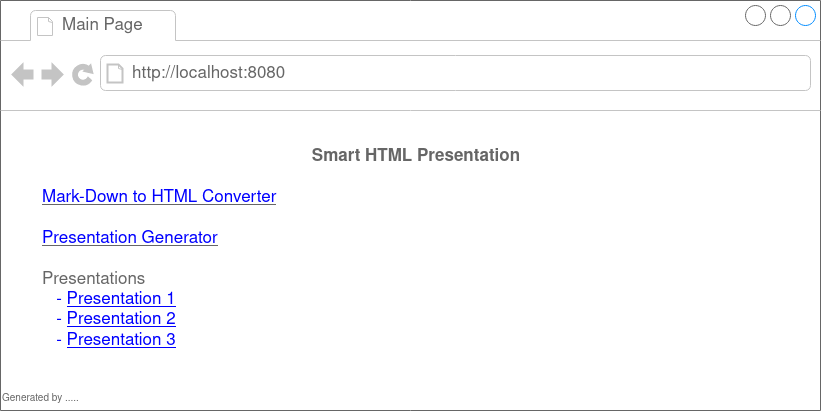
\includegraphics[scale=0.31]{Mockups/MainPage.png}}
    \caption{Main Page}
\end{figure}


\subsection{Mark-Down to HTML Generator}

Mark-Down to HTML part consist of 3 parts. In the top bar, new generated page name and location is to be determined. Also the container consist of save button to save generated HTML page. The main part is consist of 2 pages. In the left part, it is expected to input MD from user and accordingly generated image will be shown in the left frame. The mock-up can be seen in figure 2.

\begin{figure}[h]
    \href{https://raw.githubusercontent.com/krmacit/SWE599-Project-Report-2021S-Macit-KerimCan/master/Mockups/MarkdownToHTML.png}{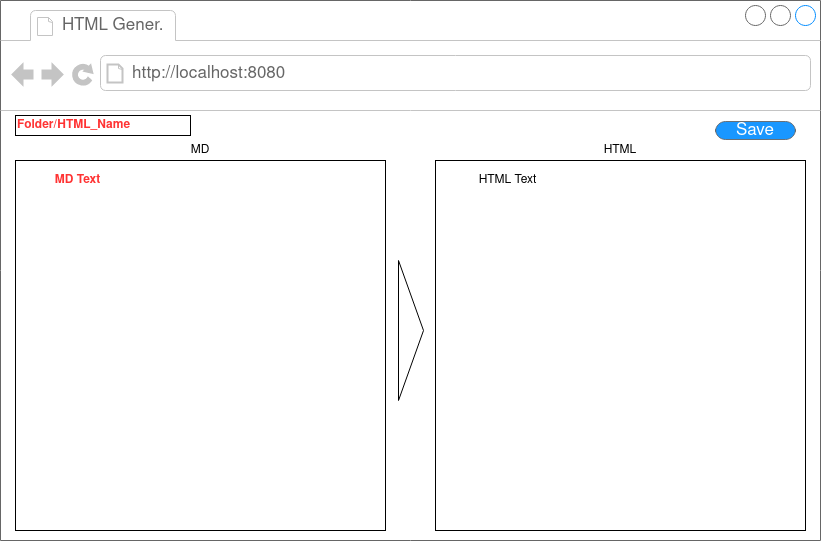
\includegraphics[scale=0.3]{Mockups/MarkdownToHTML.png}}
    \caption{Slide Page}
\end{figure}

\subsection{Presentation Generator}

The presentation generator has also similar top bar, generated presentation name and save button. In the main part of the page, all generated pages is shown with grouping according to containing folder. Each presentation has also input form which shows the slide order.

The system will generate the presentation with inputted order. The system does not allow user to give same order number to more than one slide.

\begin{figure}[h]
    \href{https://raw.githubusercontent.com/krmacit/SWE599-Project-Report-2021S-Macit-KerimCan/master/Mockups/PresentationGenerator.png}{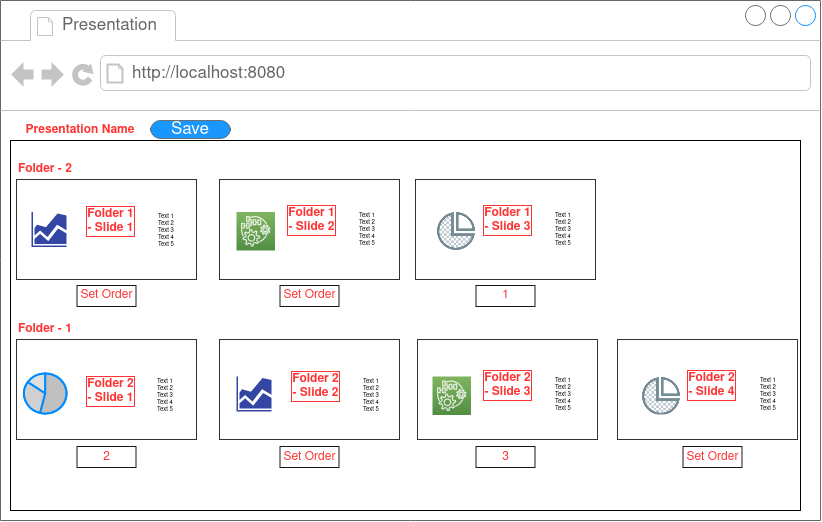
\includegraphics[scale=0.3]{Mockups/PresentationGenerator.png}}
    \caption{Presentation Generator Page}
\end{figure}

\subsection{Presentation Navigation System}

Last part of the system is navigation system. The system shows navigation tools, forward and backward button. The buttons in the below has also table of content system. The page mock-up can be seen in figure 2. These buttons are visible only when the mouse button hovers towards it, otherwise it will be invisible.

\begin{figure}[h]
    \href{https://raw.githubusercontent.com/krmacit/SWE599-Project-Report-2021S-Macit-KerimCan/master/Mockups/NavigationSystem_1.png}{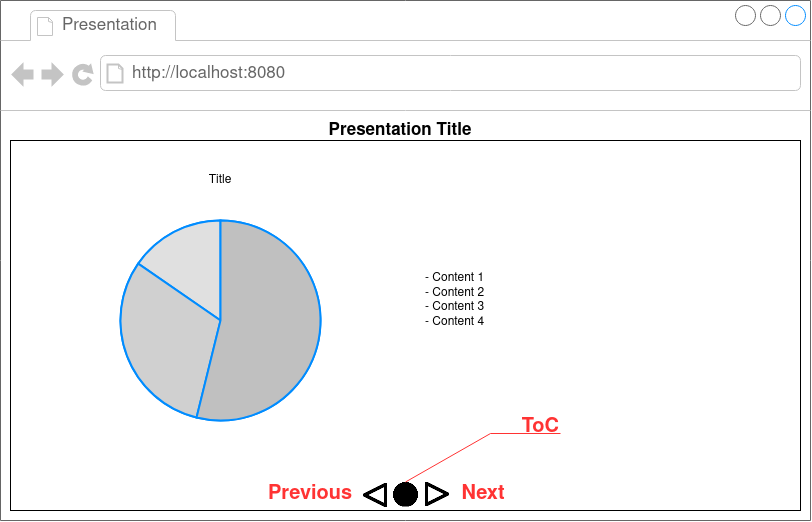
\includegraphics[scale=0.32]{Mockups/NavigationSystem_1.png}}
    \caption{Presentation Navigation Page}
\end{figure}

The table of content will be opened over current presentation page. It shows all the pages the presentation consists. Selecting any page will direct to that page. 

\begin{figure}[h]
\href{https://raw.githubusercontent.com/krmacit/SWE599-Project-Report-2021S-Macit-KerimCan/master/Mockups/NavigationSystem_2.png}{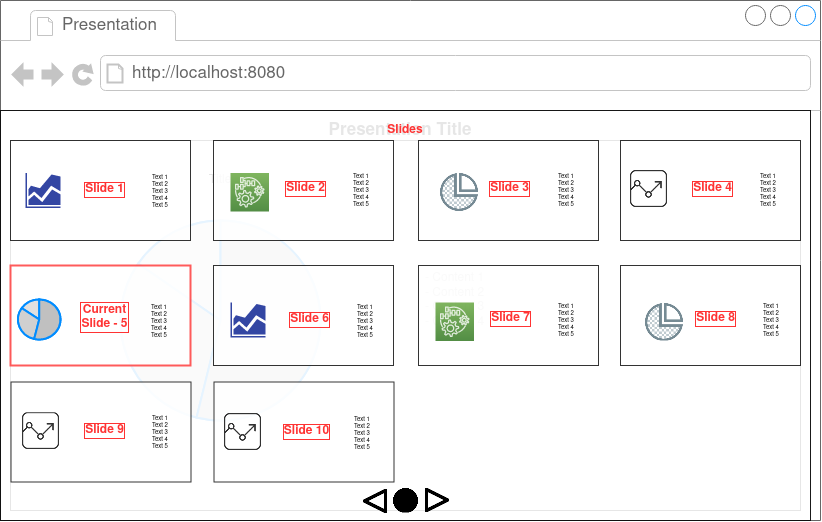
\includegraphics[scale=0.315]{Mockups/NavigationSystem_2.png}}
    \caption{Table of Content Page}
\end{figure}

\section{Implementation}
Implementation details will be added here.

\section{Demonstration}
Demonstration will be here.

\section{Conclusion}
The conclusion will be here.


% \appendices
% \section{Proof of the First Zonklar Equation}
% 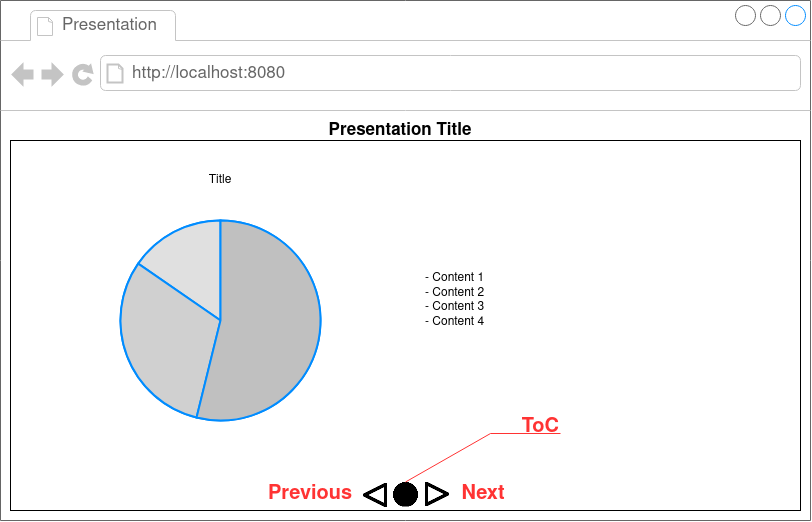
\includegraphics[scale=0.2]{Mockups/NavigationSystem_1.png}

% Proof of the First Zonklar Equation


% use section* for acknowledgment
% \section*{Acknowledgment}


% The authors would like to thank...


% \ifCLASSOPTIONcaptionsoff
%   \newpage
% \fi

% \IEEEtriggeratref{32}
% \bibliographystyle{IEEEtran}
% \bibliography{IEEEabrv,bingol-PaperTemplateIEEE}

\end{document}


